\documentclass[a4 paper]{article}
% Set target color model to RGB
\usepackage[inner=2.0cm,outer=2.0cm,top=2.5cm,bottom=2.5cm]{geometry}
\usepackage{setspace}
\usepackage[rgb]{xcolor}
\usepackage{verbatim}
\usepackage{subcaption}
\usepackage{amsgen,amsmath,amstext,amsbsy,amsopn,tikz,amssymb,tkz-linknodes}
\usepackage{fancyhdr}
\usepackage[colorlinks=true, urlcolor=blue,  linkcolor=blue, citecolor=blue]{hyperref}
\usepackage[colorinlistoftodos]{todonotes}
\usepackage{rotating}
%\usetikzlibrary{through,backgrounds}
\hypersetup{%
pdfauthor={Ashudeep Singh},%
pdftitle={Homework},%
pdfkeywords={Tikz,latex,bootstrap,uncertaintes},%
pdfcreator={PDFLaTeX},%
pdfproducer={PDFLaTeX},%
}
%\usetikzlibrary{shadows}
% \usepackage[francais]{babel}
\usepackage{booktabs}
\newcommand{\ra}[1]{\renewcommand{\arraystretch}{#1}}

\newtheorem{thm}{Theorem}[section]
\newtheorem{prop}[thm]{Proposition}
\newtheorem{lem}[thm]{Lemma}
\newtheorem{cor}[thm]{Corollary}
\newtheorem{defn}[thm]{Definition}
\newtheorem{rem}[thm]{Remark}
\numberwithin{equation}{section}

\newcommand{\homework}[6]{
   \pagestyle{myheadings}
   \thispagestyle{plain}
   \newpage
   \setcounter{page}{1}
   \noindent
   \begin{center}
   \framebox{
      \vbox{\vspace{2mm}
    \hbox to 6.5 in { {\bf CSE 202: Design and Analysis of Algorithms \hfill {\small (#2)}} }
       \vspace{6mm}
       \hbox to 6.5 in { {\Large \hfill #1  \hfill} }
       \vspace{6mm}
       \hbox to 6.5 in { {\it Instructor: {\rm #3} \hfill Name: {\rm #5}, Netid: {\rm #6}} }
       %\hbox to 6.28in { {\it TA: #4  \hfill #6}}
      \vspace{2mm}}
   }
   \end{center}
   \markboth{#5 -- #1}{#5 -- #1}
   \vspace*{4mm}
}

\newcommand{\problem}[2]{~\\\fbox {\textbf{Problem #1}}\newline\newline } %\hfill (#2 points)\newline\newline}
\newcommand{\problemdes}{~\newline \textbf{Problem Description}\newline}
\newcommand{\subproblem}[1]{~\newline\textbf{(#1)}\newline}
\newcommand{\D}{\mathcal{D}}
\newcommand{\Hy}{\mathcal{H}}
\newcommand{\VS}{\textrm{VS}}
\newcommand{\solution}{~\newline\textbf{\textit{Solution}}}
\newcommand{\subsolution}[1]{~\newline\textbf{(#1)}\newline}

\newcommand{\bbF}{\mathbb{F}}
\newcommand{\bbX}{\mathbb{X}}
\newcommand{\bI}{\mathbf{I}}
\newcommand{\bX}{\mathbf{X}}
\newcommand{\bY}{\mathbf{Y}}
\newcommand{\bepsilon}{\boldsymbol{\epsilon}}
\newcommand{\balpha}{\boldsymbol{\alpha}}
\newcommand{\bbeta}{\boldsymbol{\beta}}
\newcommand{\0}{\mathbf{0}}

% =============== pseudo code package ===============
\usepackage[linesnumbered,ruled,vlined]{algorithm2e}%[ruled,vlined]{
\usepackage{algpseudocode}
\usepackage{amsmath}
\renewcommand{\algorithmicrequire}{\textbf{Input:}}  % Use Input in the format of Algorithm
\renewcommand{\algorithmicensure}{\textbf{Output:}} % Use Output in the format of Algorithm

\begin{document}
\homework{Homework \#1}{Due: 10/19/19}{Ramamohan Paturi}{}{Shihan Ran}{A53313589}

\newpage
\problem{1: Maximum weight subtree} % {10+10+10+20=50}

\problemdes

The maximum weight subtree is as follows. You are given a tree $T$ together with (not necessarily positive) weights $w(i)$ for each node $i \in T$. A subtree of $T$ is any connected subgraph of $T$, (so a subtree is not necessarily the entire subtree rooted at a node). You wish to find a subtree of $T$ that maximizes $\sum_{i \in S} w(i)$. Design an efficient algorithm for solving this problem. Note that there is a linear (in the number of nodes of the tree) time algorithm for this problem. You can assume that for each node in the tree $T$, you are given a list of its children as well as the parent pointer (except for the root node).

\solution

\subsolution{High-level description}

Assume for each node of this tree, it at most has $m$ children nodes. Our solution is to do a tree traversal. At each node, we iterate all the children nodes and find their subtree value. Then the value of subtree rooted at the current node is equal to the sum of current node value and the subtree values of all $m$ children nodes. After getting the current subtree weight sum, we compare it with the stored maximum value and take the largest.

\subsolution{Pseudo Code}

\begin{algorithm}[]
  \caption{Maximum weight subtree}
  \KwIn{root node $root$}
  \KwOut{$maxWeightSum$}
  \If{$root$ is not valid}
  {
  	return $0$\;
  }
  initialize $maxWeightSum$ as the min value of the integer, say, $-\inf$\;
  $findMaxWeightSum(root, maxWeightSum)$\;
  return $maxWeightSum$\;
\end{algorithm}

\begin{algorithm}[]
  \caption{Find max weight sum}
  \KwIn{root node $root$, $maxWeightSum$}
  \KwOut{$maxWeightSum$}
  \If{$root$ is not valid}
  {
  	return $0$\;
  }
  weightSum = root.value\;
  \For{child in root.children}
  {
  	$weightSum = weightSum + findMaxWeightSum(child, maxWeightSum)$
  }
  $maxWeightSum = \max(maxWeightSum, weightSum)$
  return $weightSum$\;
\end{algorithm}


\subsolution{Correctness}

We update $maxWeightSum$ each time we use $findMaxWeightSum(root, maxWeightSum)$ function to find a maximum weight sum. Every time we calculate the weight sum, we compare it with the maximum weight sum we've seen so far.

The weight sum at each node is computed as root weight plus all the children's weights. There are two cases, 

1. The root's weight is positive. Then indeed, the maximum weight sum should plus node weight.

2. The root's weight is negative. Then the maximum weight sum is one of the children's maximum weight sum. We'll update the $maxWeightSum$ when we iterate the $findMaxWeightSum$ function to compute children's value.

Also, our algorithm terminates. It returns 0 for leaf's children node value if the node is a leaf node. Thus, it's correct.

\subsolution{Time complexity}

Since the tree traversal only visits each node once, hence the time complexity is $O(n)$, and $n$ is the number of nodes.

We can also interpret the complexity as the following recursion tree: 

$T(n) = m*T(n/m)+ c$.

And the second step is $T(n/m) = m*T(n/(m^2)) + c$, thus $T(n) = m^2*T(n/(m^2)) + 2c + c$ ...

And the last step is $T(n) = n*T(1) + c(1+m^1+...m^h)$, with h is the hight of the recursion tree $h = \log_m(n)$.

So the time complexity is $O(n*c + c*(m^(h+1)-1)/(m-1)) = O(n)$



\newpage
\problem{2: Remote Sensors} % {10+10+10+20=50}

\problemdes

\begin{figure}[!ht]
    \centering
    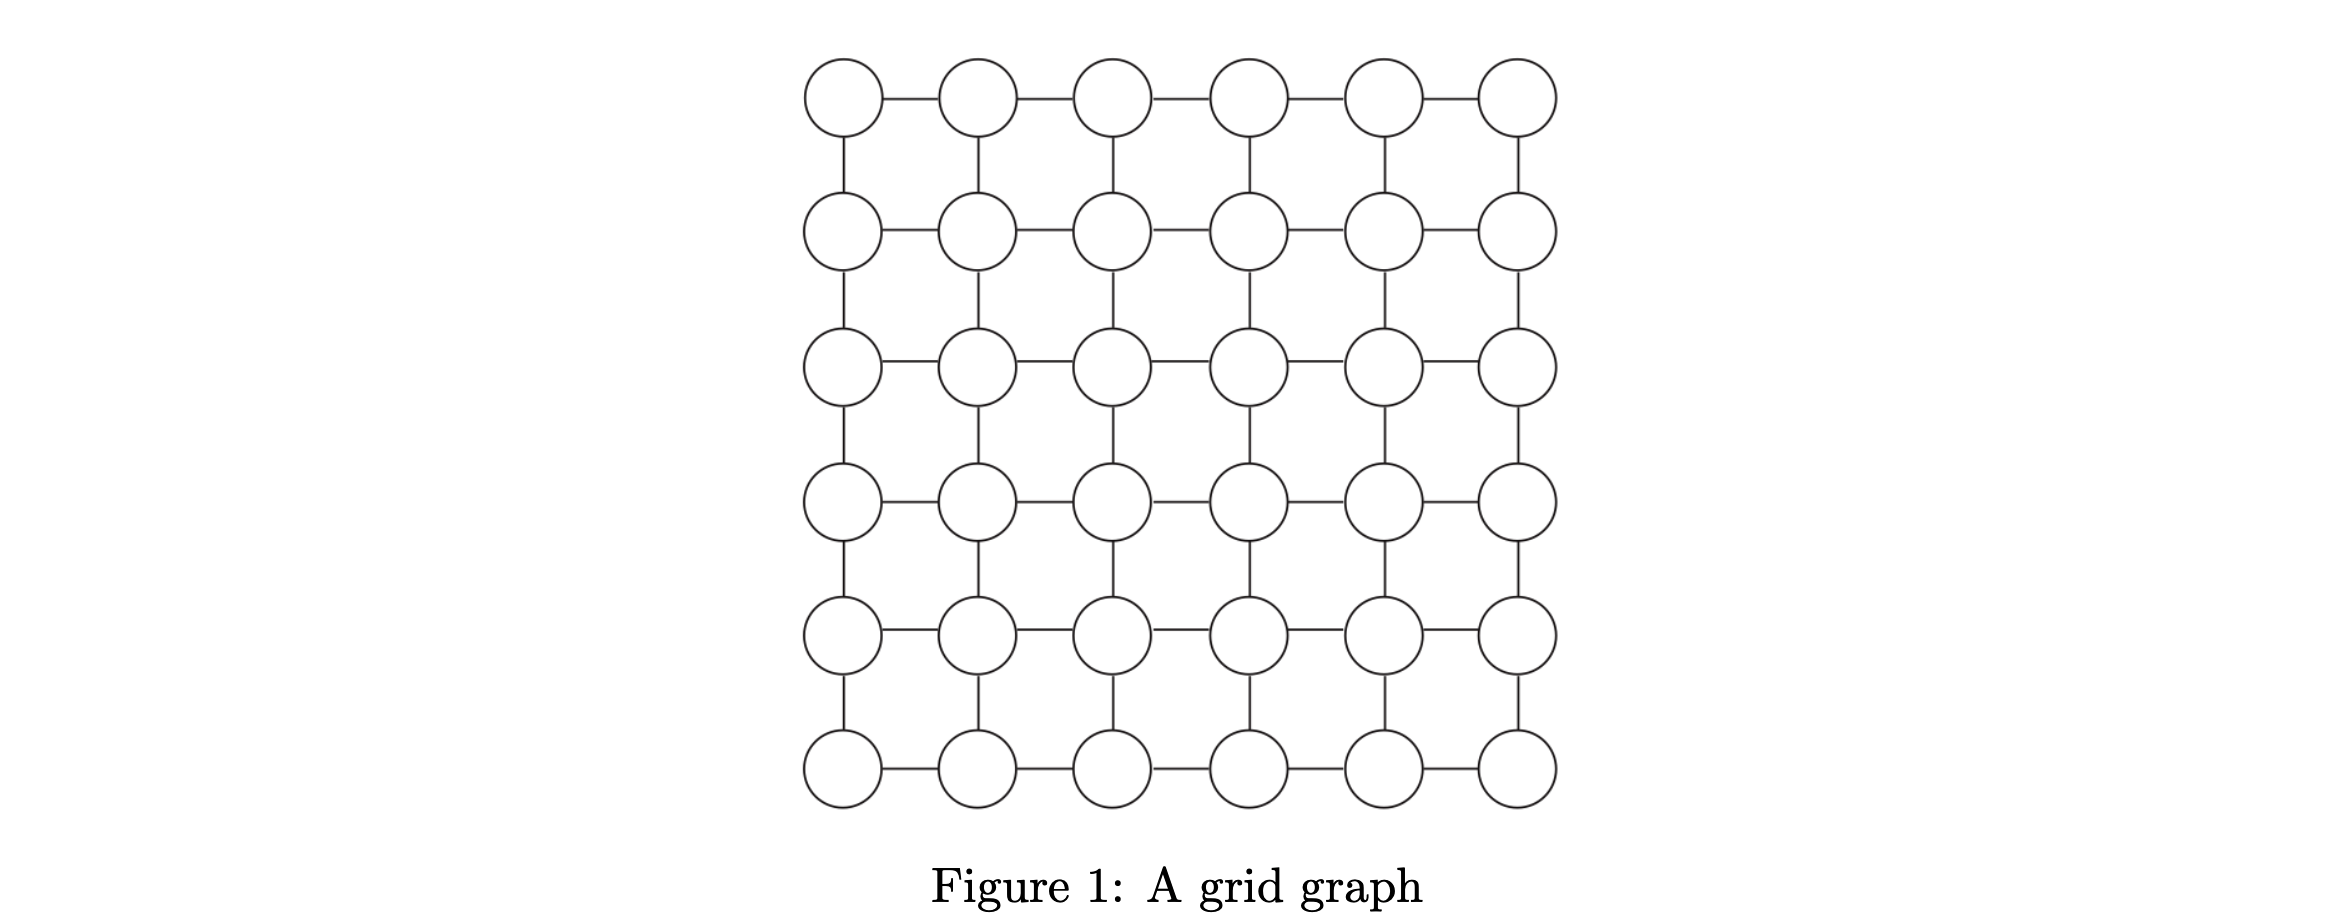
\includegraphics[width=\textwidth]{graph.png}
    \label{fig:algo}
\end{figure}

Suppose you are given an $n \times n$ grid graph $G$, as in Figure 1 Associated with each node $v$ is a weight $w(v)$, which is a nonnegative integer. You may assume that the weights of all nodes are distinct. Your goal is to choose an independent set $S$ of nodes of the grid, so that the sum of the weights of the nodes in $S$ is as large as possible. (The sum of the weights of the nodes in $S$ will be called its total weight.) Consider the following greedy algorithm for this problem.

\begin{figure}[!ht]
    \centering
    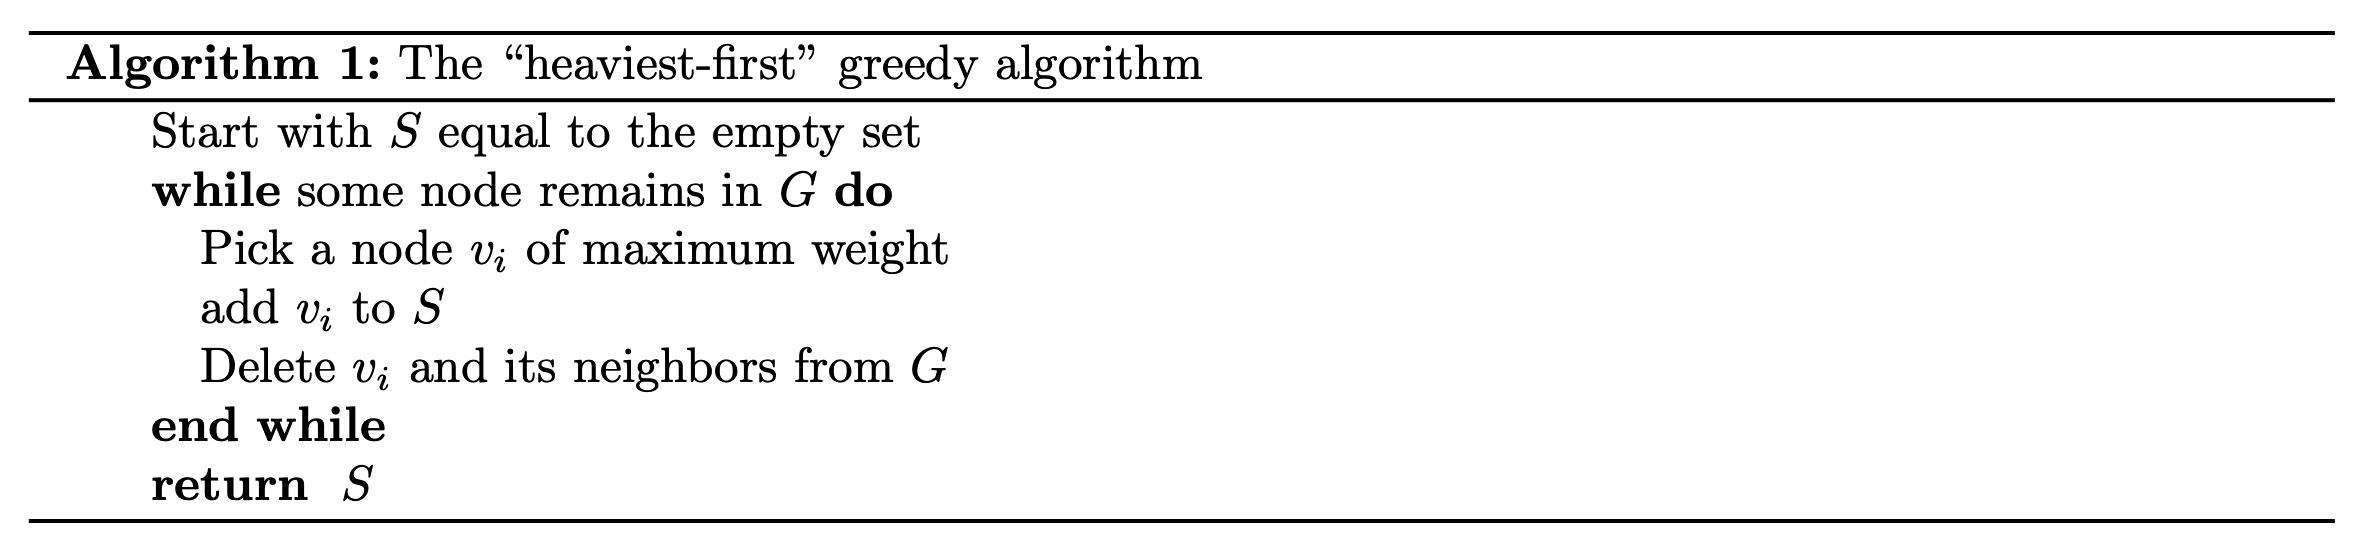
\includegraphics[width=\textwidth]{algorithm.png}
    \label{fig:algo}
\end{figure}

\subproblem{Subproblem 1}

Let $S$ be the independent set returned by the “heaviest-first” greedy algorithm, and let $T$ be any other independent set in $G$. Show that, for each node $v \in T$, either $v \in S$,or there is a node $v^\prime \in S$ so that $w(v) \le w(v^\prime)$ and $(v, v^\prime)$ is an edge of $G$.

\subsolution{Solution 1}

%\subsolution{High-level description}

%\subsolution{Pseudo Code}

% \subsolution{Correctness}


% \subsolution{Time complexity}

\textit{Proof.} For node $v\in T$, if $v \notin S$, then it means that it is deleted at some iteration when selecting its neighbor $v^\prime$. And following the instruction of greedy algorithm, $v^\prime$ must contain a larger weight than $v$. Otherwise we will choose to add $v$ to $S$. Hence, we proved that for each node $v\in T$, either $v\in S$ or there is a node $v^\prime \in S$ so that $w(v) \le w(v^\prime)$ and $(v, v^\prime)$ is an edge of $G$.

\subproblem{Subproblem 2}

Show that the “heaviest-first” greedy algorithm returns an independent set of total weight at least $1/4$ times the maximum total weight of any independent set in the grid graph $G$.

\subsolution{Solution 2}

%\subsolution{High-level description}

%\subsolution{Pseudo Code}

%\subsolution{Correctness}

%\subsolution{Time complexity}

We use $T$ to denote any independent set in the grid graph $G$, let $S$ denote the independent set found by the heaviest-first greedy algorithm. We want to show that $W_S \ge \forall_{T} \frac{1}{4} W_{T}$.

% We need to notice that both $T$ and $S$ are independent set, which means for each node $v \in T$, its neighbors $v^\prime \notin T$. 

For any node $v \in T$, 

\textit{Case 1}. If $v\in S$, since $G$ is a grid graph, then at most four neighboring nodes of no greater weights $v^\prime_{1, 2, 3, 4} \in T$.

\textit{Case 2}. If $v\notin S$, as proved in subproblem 1, there must be a node $v^\prime \in S$ so that $w(v) \le w(v^\prime)$ and $(v, v^\prime)$ is an edge of $G$. For $v^\prime$, there are at most four neighboring nodes of no greater weights $\in T$.

Either case, the total weight of all nodes in $T$ should not be greater than four times than the total weights of all nodes in $S$. Hence, we proved that $W_S \ge \forall_{T} \frac{1}{4} W_{T}$.











\newpage
\problem{3: Largest set of indices within a given distance} % {10+10+10+20=50}

\problemdes

You are given a sequence of numbers $a_{1}, \dots, a_{n}$ in an array. You are also given a number k. Design an efficient algorithm to determine the size of the largest subset $L \subseteq\{1,2, \cdots, n\}$ of indices such that for all $i, j \in L$ the difference between $a_i$ and $a_j$ is less than or equal to $k$. There is an $O(n \log n)$ algorithm for this problem.
For example, consider the sequence of numbers $a_1 = 7,a_2 = 3,a_3 = 10,a_4 = 7,a_5 = 8,a_6 = 7,a_7 = 1,a_8 = 15,a_9 = 8$ and let $k = 3$. $L = \{1,3,4,5,6,9\}$ is the largest such set of indices. Its size is 6.

\solution

\subsolution{High-level description}

Since we only need to determine the size of the largest subset L instead of determining the subset L itself, indexes are not so important then. What we really care about is the differences between elements and the max differences should be less than or equal to $k$. 

Thus, we can sort this array first, and then iterate through the sorted array, find out the maximum length of continuous elements with a maximum difference less than or equal to $k$. 

One tricky thing is how to find the maximum length efficiently. Our solution is using two pointers, the left one stays at index $i$ and the right one points to index $j$. We have $i<j, A[i]<=A[j]$. 

\begin{itemize}
\item While $A[j]-A[i]<=k$, we shift our right pointer. 
\item Compare the current length $j-i$ with the longest size we've seen before, and take the maximum of these two values.
\item Shift the left pointer to $i+1$, since our array is sorted, then $A[i+1]>=A[i]$, which means $A[j]-A[i+1]<=k$ still stands. However this time the length is $j-(i+1)$, and it must be less than the maximum value we just got. Hence, we can shift our right pointer to find the newest index $j'$.
\item Go to Step 1.
\end{itemize}

After iterate through the whole array, we will get the maximum length $size$.

\subsolution{Pseudo Code}

\begin{algorithm}
  \caption{Largest set of indices within a given distance}
  \KwIn{$A$ as an array, $k$}
  \KwOut{$size$}
  sort the input array $A$\;
  initialize size as min value of integer, say, $-\inf$\;
  $leftPointer = 1, rightPointer = 1$\;
  \While{$rightPointer <= len(A)$}
  {
    \While{$A[rightPointer]-A[leftPointer]<=k$}
    {
    	$rightPointer = rightPointer + 1$\;
    }
    $size = \max(size, rightPointer-leftPointer)$\;
    $leftPointer = leftPointer +1$\;
}
    return $size$\;
\end{algorithm}

\subsolution{Correctness}

\subsolution{Time complexity}

The sorting algorithm can take $O(n\log n)$ time complexity. As for the remaining part, for both left pointer and right pointer, we only need to iterate through the array once, hence it's $O(n)$ time complexity.

Overall, it's $O(n\log n)$.




\newpage
\problem{4: Cellular network} % {10+10+10+20=50}

\problemdes

Consider the problem of selecting nodes for a cellular network. Any number of nodes can be chosen from a finite set of potential locations. We know the benefit $b_i \geq 0$ of establishing site i. However, if sites i and j are selected as nodes, then the benefit is offset by $c_{ij}$, which is the cost of interference between the two nodes. Both the benefits and costs are non-negative integers. Find an efficient algorithm to determine the subset of sites as the nodes for the cellular network such that the sum of the node benefits less the interference costs is as large as possible.

Design an efficient polynomial-time algorithm.

Provide a high-level description of your algorithm, prove its correctness, and analyze its time complexity.

\solution

\subsolution{High-level description}

\subsolution{Pseudo Code}

\subsolution{Correctness}

\subsolution{Time complexity}







\end{document} 
